\section{L09-Trasmissione del calore}
La \textbf{trasmissione del calore} si occupa dello studio dell’insieme delle leggi che governano il passaggio di calore da un sistema ad un altro o da un punto ad un altro di uno stesso sistema, dei dispositivi coinvolti negli scambi di calore e delle leggi che danno la distribuzione di temperatura all’interno di un sistema in funzione dello spazio e del tempo.\newline
\newline
Obiettivi della seconda parte del corso:
\begin{itemize}
    \item Determinare il calore scambiato tra un punto ed un altro;
    \item Determinare la distribuzione di temperatura nei vari punti ed eventualmente la sua variazione nel tempo;
\end{itemize}
\subsection{Concetti base}
\subsubsection{Calore scambiato}
Nel \textbf{caso generale}, la quantità di \textbf{calore} scambiata tra due sistemi, $Q$, durante
un \textbf{intervallo di tempo}, $\Delta t$, è data dall’integrale temporale della \textbf{potenza
istantanea}, $\dot{Q}$, tra l’istante $t$ e l’istante $t + \Delta t$
\[
    Q = \int_{t}^{t+\Delta t} \dot{Q}dt
\]
Nel \textbf{caso particolare} in cui $\dot{Q}=$ costante $\rightarrow Q = \dot{Q} \cdot \Delta t$
\subsubsection{Flusso termico}
Si definisce \textbf{flusso termico} la potenza riferita ad una superficie di area
unitaria. Il flusso termico medio su una superficie si esprime come:
\[
    J = \frac{\dot{Q}}{A} \left[\frac{W}{m^2}\right] \;\;\;\;\;\;\;\;\;\;\text{flusso termico areico}\;
\]
Il \textbf{flusso termico} puà essere definito dalla realzione:
\[
    J = f(\text{parametro}, \Delta t) \left[\frac{W}{m^2}\right]
\]
dove $\Delta t$ è una differenza di temperature e dove per "\textbf{parametro}" si intende: coefficiente che tiene conto della maggiore o minore facilità con la quale, a parità di $\Delta t$, ha luogo il trasferimento di calore (per noi questo parametro prenderà nomi come resistenza, conduttanza, trasmittanza).\newline
\newline
Di seguito vedremo le vaire forme che assume l'espressione del flusso termico a fronte dei diversi meccanismi che lo scaturiscono.
\subsubsection{La conduzione}
La \textbf{conduzione} è il trasferimento di energia che si verifica per effetto dell’interazione delle
particelle di una sostanza dotata di maggiore energia con quelle adiacenti dotate
di minore energia.\newline
\newline
Può avvenire:
\begin{itemize}
    \item nei liquidi;
    \item nei solidi;
    \item nei gas.
\end{itemize}
(non nel vuoto...)
\ \newline
\textbf{Postulato di Fourier}:
\[
    \vec{J} = - k \nabla T \;\;\;\;\;\;\;\;\;\;\;\;\;\;\; \nabla T \rightarrow grad(T)
\]
dove $k$ è la \textbf{conduttività termica}. Inoltre notiamo che il flusso termico è espresso come un vettore che ha quindi un verso (dovuto alla presenza del gradiente di $T$).\newline
\newline
\textbf{es.} Potenza termica trasmessa per conduzione attraverso una lastra piana indefinita di spessore costante:
\[
    \dot{Q}_{COND} =  - k A \frac{\Delta T}{\Delta x}
\]
con $\dot{Q}_{COND}$ potenza termica; $k$ conduttività termica; $A$ superficie normale; $\Delta x$ spessore; $\Delta T$ differenza di temperatura
\subsubsection{La convezione}
La \textbf{convezione} è il trasferimento di energia tra una superficie solida e un fluido adiacente in
movimento.
\begin{itemize}
    \item Implica gli effetti combinati di conduzione e trasporto di massa;
    \item Il calore trasmesso per convezione aumenta all'aumentare della velocità del fluido.
\end{itemize}
\ \newline
\textbf{Convezione forzata}:\newline
Avviene quando il fluido è forzato a scorrere su una superficie da mezzi esterni (ad esempio un ventilatore).\newline
\newline
\textbf{Convezione naturale (o libera)}:\newline
Avviene quando il moto del fluido è causato da forze ascensionali che sono indotte dalle differenze di densità dovute alla variazione di temperatura del fluido in un campo gravitazionale.\newline
\newline
La potenza termica trasmessa per convesione è espressa dalla \textbf{legge di Newton}:
\[
    \vec{J} = h (T_p - T_{\infty})
\]
dove $h$ è il coefficiente di scambio termico convettivo ($[W/m^2K]$), che è un parametro molto incerto solitamente; $T_p$ è la temperatura della parete solida ($[K]$); $T_{\infty}$ è la temperatura del fluido ($[K]$).\newline
\newline
\textbf{es.} Potenza termica trasmessa per convezione da una lastra piana indefinita lambita da aria oppure acqua:
\begin{center}
    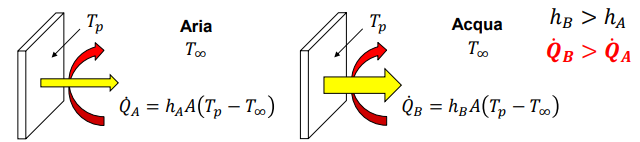
\includegraphics[height=3cm]{../L09/img1.PNG}
\end{center}
\subsubsection{L'irraggiamento}
E’ il trasferimento di energia che avviene attraverso le onde elettromagnetiche (o
fotoni) prodotte da variazioni nelle configurazioni elettroniche degli atomi e delle
molecole.\newline
\newline
Ad esempio, il sole trasferisce l'energia alla terra per irraggiamento.\newline
\begin{itemize}
    \item Non richiede la presenza di un mezzo interposto (quindi avviene anche nel vuoto);
    \item Avviene alla vellocità della luce;
    \item Tutti i corpi a temperatura superiore allo zero assoluto ($0 k$) emettono radiazione termica.
\end{itemize}
\ \newline
La potenza massima termica trasmessa per irraggiamento da una superficie a temperatura assoluta $T_s [k]$ è data dalla \textbf{legge di Stegan Boltzmann}:\newline
La legge di Stefan Boltzman afferma che la potenza trasmessa da un'area $A$ di un corpo ideale (detto corpo nero) è 
\[
    \dot{Q}_{e, max} = \sigma_{0} A (T_S)^4
\]
dove $\sigma_{0} = 5,67 \cdot 10^{-8} [W/m^2K^4]$ è la \textbf{costante di Stefan Boltsmann}.\newline
\newline
Nel momento in cui non siamo più in un caso ideale possiamo usare la seguente relazione.\newline
\textbf{Potenza emessa per irraggiamento}:\newline
La potenza emessa per irraggiamento da una qualsiasi superficie reale è invece data dalla realzione
\[
    \dot{Q}_e = \epsilon \sigma_{0} A (T_s)^4
\]
dove $\epsilon$ è l' \textbf{emissività} della superficie il cui valore, compreso tra $0$ e $1$, è la misura di quanto il comportamento di una superficie si approssima a quella del corpo nero, per il quale $\epsilon = 1$.\newline
\newline
Poichè nei corpi reali non tutta la radiazione elettromagnetica incidente viene riflessa si definisce come \newline
\textbf{Potenza termica netta per irraggiamento}:\newline
la differenza tra la potenza termica radiante emessa e quella assorbita da una superficie.\newline
\newline
La determinazione della potenza termica netta scambiata è complessa in quanto dipende da numerosi fattori quali:
\begin{itemize}
    \item Proprietà delle superfici;
    \item Orientamento relativo;
    \item Caratteristiche del mezzo tra le ddeu superfici che irraggiano.
\end{itemize}
\ \newline
 \textbf{es.} Nel caso di una superficie piccola è semplice: $\dot{Q}_{irr} = \epsilon \sigma_{0} A (T_S^4 - T_C^4)$ (notare l'elevamento alla quarta che è delle singole temperature e non di tutta la parentesi).